\section{Sonnet to the Knight}

\begin{figure}[h]
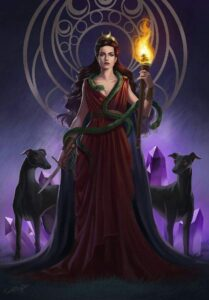
\includegraphics[width=.4\textwidth]{HecateWithHounds-209x300.jpg}
\end{figure}

\begin{verse}
Born in ignorance, and tempted by sin\\ Aroused by beauty and to passions bound\\ Love and adventure, the knight has found,\\ Not in the world for the struggle's within.

The greater battle is by far the best;\\ In Napoli he lay dying in bed\\ Ere his journey to the home of the dead\\ Ridwan assures that he has passed the test.

A glowing torch in the moonlighted sky\\ Guides the knight on the path to the river\\ Howling hounds tell him the goddess is nigh

Hecate assuages his hidden fear.\\ At the crossroads she will him deliver,\\ There she will whisper his poem in God's ear.
\end{verse}
\url{https://www.gornahoor.net/library/OdeToTheKnight.mp3}



\flrightit{Posted on 2021-02-19 by Cologero}

\begin{center}* * *\end{center}

\begin{footnotesize}
\begin{sffamily}
\texttt{Rusalka on 2021-02-20 at 10:02 said:}

Thank you ?. May Beauty always follow you.

\hfill

\texttt{Rusalka on 2023-05-21 at 16:25 said:}

My dearest Knight, I whispered \& spoke your poem. I unlocked the door, and not for a moment were you alone.

Be well and stay well, I shall remember \& pray until my last breath.

May the heavenly choirs sing \& perform for you.

\hfill

\texttt{Rusalka on 2023-05-21 at 16:32 said:}

She spoke his poem into God's ear

And even God's unmoved eye let out a tear.

Not for a moment were you alone, my Knight. Shine like a blazing Sun and keep me ablaze here.

\end{sffamily}
\end{footnotesize}

